Our last topic is \emph{randomised linear algebra}: how can we incorporate random matrices into developing better algorithms for linear algebra? Numerical linear algebra (that is to say, linear algebra done on computer using algorithms) underlies much of modern computational mathematics, including the numerical solution of Partial Differential Equations (PDEs). Recently, incorporating randomness into numerical linear algebra has become a tool to design algorithms that can scale to much larger problems than non-randomised algorithms. For example, Stochastic Gradient Descent is a randomised version of a linear algebra algorithm (Gradient Descent, or in the linear case Conjugate Gradients) that underlies training of Neural Networks in Machine Learning. Without randomness, training can get stuck in local minima, and so it is absolutely essential.

In this section we will focus on a much simpler problem which can in many ways be viewed as a baby version of training a Neural Network: linear regression. (Indeed, linear regression can be thought of as a "one-layer" Neural Network.)  We will first review least squares, where rectangular systems are ``solved'' by finding a vector that minimises the error in norm, with linear regression being a classic application. We then explore experimentally how using a random \emph{sketch matrix} can substantially reduce the sizes of matrices involved, and by averaging over multiple sketches we can obtain a good approximation to the true least squares system. 

\textbf{Further Reading}  For simplicity we focus on experimental implementation and observation of randomised linear algebra, but  \href{https://www.cambridge.org/core/services/aop-cambridge-core/content/view/4486926746CFF4547F42A2996C7DC09C/S0962492920000021a.pdf/div-class-title-randomized-numerical-linear-algebra-foundations-and-algorithms-div.pdf}{Martinsson \& Tropp 2020} gives  an overview of the mathematical proofs of what we observe. It also discusses some other simple problems that could form good posters like trace estimation (approximating the trace of a matrix without evaluating every single diagonal). Randomised linear algebra is a very active research area and so there will probably be a lot of progress in the next few years.

\section{Least squares}
We begin with an introduction to least squares.  For a rectangular matrix $A \ensuremath{\in} \ensuremath{\bbR}^{m \ensuremath{\times} n}$ with $m > n$ and a right-hand side $\ensuremath{\bm{\b}} \ensuremath{\in} \ensuremath{\bbR}^m$ we cannot solve $A \ensuremath{\bm{\c}} = \ensuremath{\bm{\b}}$ unless $\ensuremath{\bm{\b}}$ happens to be in the column span of $A$. However, we can instead find $\ensuremath{\bm{\c}} \ensuremath{\in} \ensuremath{\bbR}^n$ that satisfies $A \ensuremath{\bm{\c}} \ensuremath{\approx} \ensuremath{\bm{\b}}$, in the sense that
\[
\| A\ensuremath{\bm{\c}} - \ensuremath{\bm{\b}}\|
\]
is minimised. This is called the \emph{least squares} solution.  Minimising a norm is equivalent to minimising its square, and expanding out we see that it is equivalent to a quadratic minimisation problem:
\[
\| A\ensuremath{\bm{\c}} - \ensuremath{\bm{\b}}\|^2 = (A\ensuremath{\bm{\c}} - \ensuremath{\bm{\b}})^\ensuremath{\top} (A\ensuremath{\bm{\c}} - \ensuremath{\bm{\b}}) = \ensuremath{\bm{\c}}^\ensuremath{\top} A^\ensuremath{\top} A \ensuremath{\bm{\c}} - 2 \ensuremath{\bm{\c}}^\ensuremath{\top} A^\ensuremath{\top} \ensuremath{\bm{\b}}  + \ensuremath{\bm{\b}}^\ensuremath{\top} \ensuremath{\bm{\b}}.
\]
In the scalar case ($n = 1$ so that $\ensuremath{\bm{\c}}$ is essentially a constant) we know we can solve this by differentiation with respect to $\ensuremath{\bm{\c}}$, and we arrive at a linear system
\[
 A^\ensuremath{\top} A \ensuremath{\bm{\c}}  =  A^\ensuremath{\top} \ensuremath{\bm{\b}}.
\]
This generalises (actually,  using linear algebra instead of calculus but we omit the details) and in general we know the least squares solution is given by
\[
\ensuremath{\bm{\c}} =  (A^\ensuremath{\top} A)^{-1} A^\ensuremath{\top} \ensuremath{\bm{\b}}.
\]
Assuming $A$ has full column rank we know $A^\ensuremath{\top} A \ensuremath{\in} \ensuremath{\bbR}^{n \ensuremath{\times} n}$ is invertible (Why?) and so this is well-posed.

A classic application of least squares is \emph{polynomial regression}. In the case of linear regression, we want to approximation data $\{b_j\}$ on a grid of points $\{x_j\}$ by a linear function $c_0 + c_1 x$. In other words, we want to solve
\[
\underbrace{\begin{bmatrix} 1 & x_1 \\
1 & x_2 \\
\ensuremath{\vdots} & \ensuremath{\vdots} \\
1 & x_n
\end{bmatrix}}_A \underbrace{\begin{bmatrix} c_0 \\
c_1
\end{bmatrix}}_{\ensuremath{\bm{\c}}} \ensuremath{\approx} \underbrace{\begin{bmatrix}
b_1 \\
b_2 \\
\ensuremath{\vdots} \\
b_n
\end{bmatrix}}_{\ensuremath{\bm{\b}}}
\]
by using the least squares solution.

Here is a depiction of the linear regression fit of (noisy) data at $n = 50$ points:


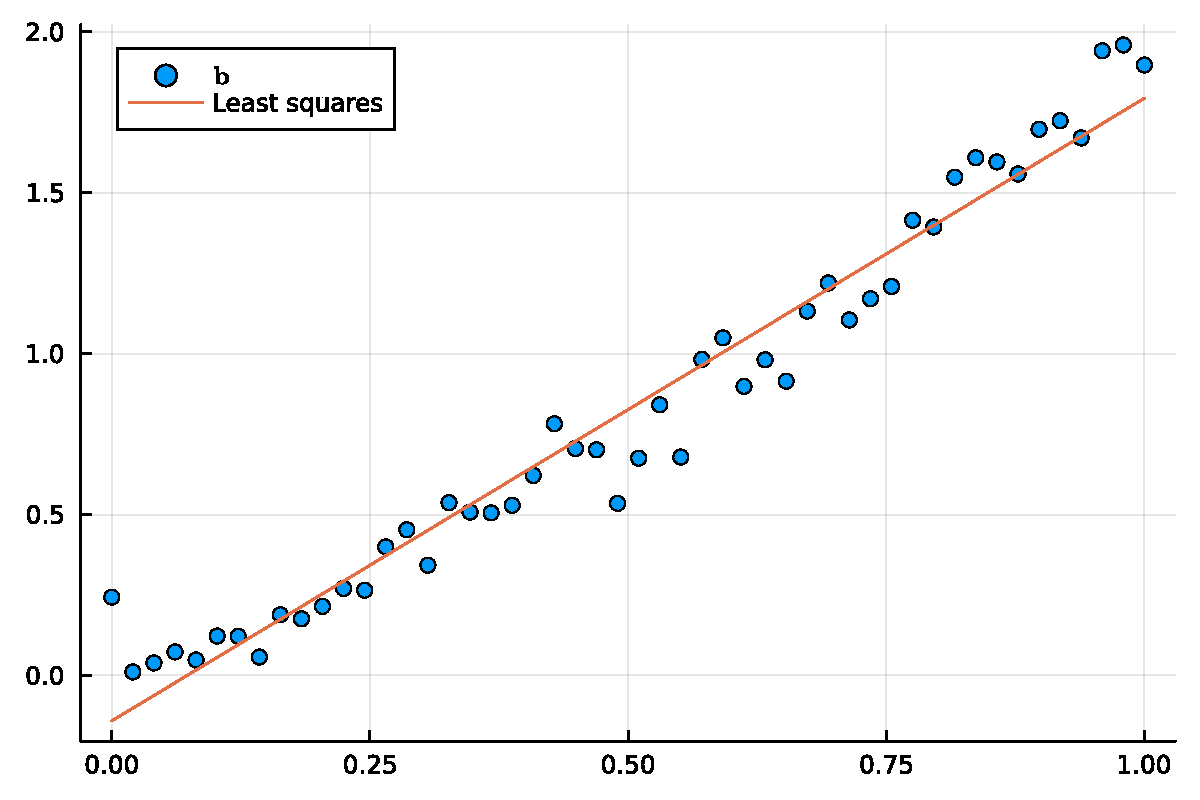
\includegraphics[width=0.6\linewidth,height=0.45\linewidth]{figures/IV.RandomisedLinearAlgebra_1_1.pdf}

\section{Randomised least squares}
In the above  data there is a lot of correlation between nearby points, hence, using every single point is unnecessary. An alternative is to \emph{sketch} the problem: use a sketch matrix $P \ensuremath{\in} \ensuremath{\bbR}^{r \ensuremath{\times} m}$ where $r \ensuremath{\ll} m$ and solve
\[
P A \ensuremath{\bm{\c}} \ensuremath{\approx} P \ensuremath{\bm{\b}}
\]
using least squares. Here we see a simple example where we use $P \ensuremath{\in} \ensuremath{\bbR}^{5 \ensuremath{\times} 50}$ with random entries:


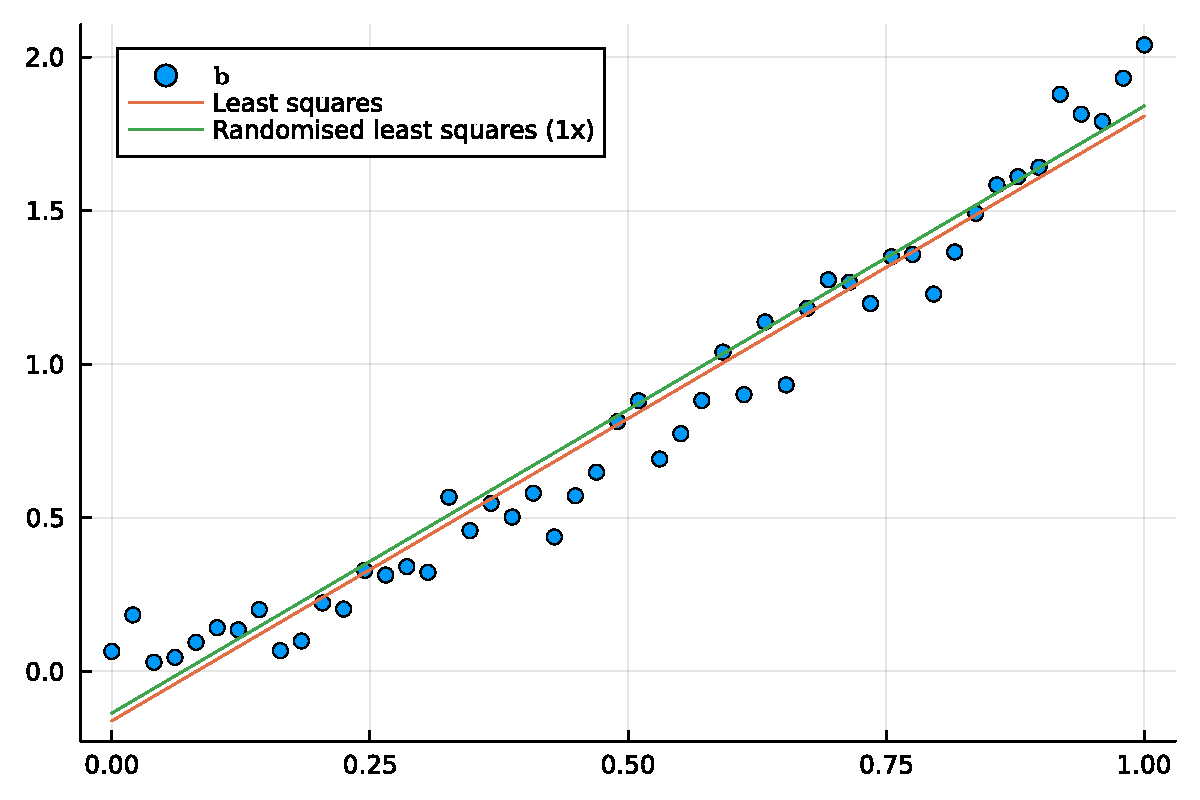
\includegraphics[width=0.6\linewidth,height=0.45\linewidth]{figures/IV.RandomisedLinearAlgebra_2_1.pdf}

This is a single sample and, to the eye, it performs fairly well even compared to the true least squares solution. Going further, we see that averaging over multiple trials is almost indistinguishable from the true least squares approximation:


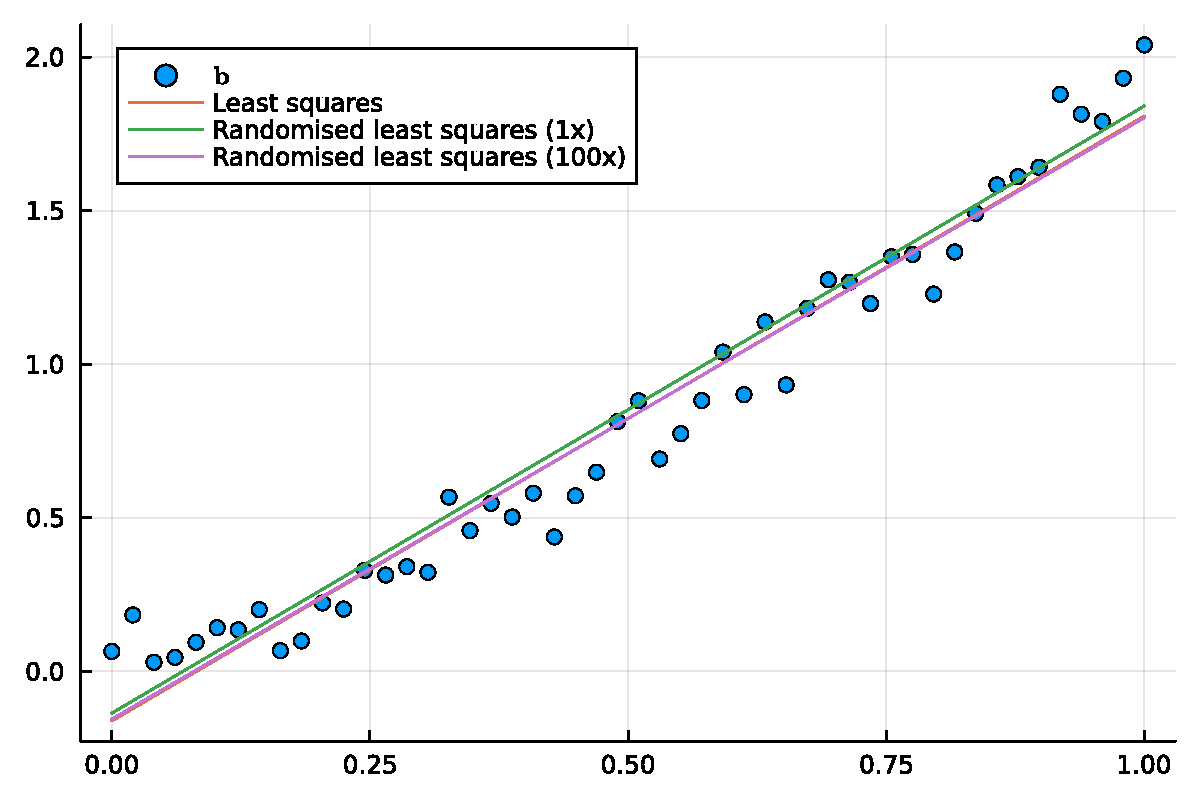
\includegraphics[width=0.6\linewidth,height=0.45\linewidth]{figures/IV.RandomisedLinearAlgebra_3_1.pdf}

Now this particular example is a bit silly: its not at all clear that solving 100 least squares systems of size $5 \ensuremath{\times} 2$ is preferred to a single least squares system of size $50 \ensuremath{\times} 2$. But we can consider a much more extreme example of $n = 10,000$. Here we compare the average over samples for varying $r$:


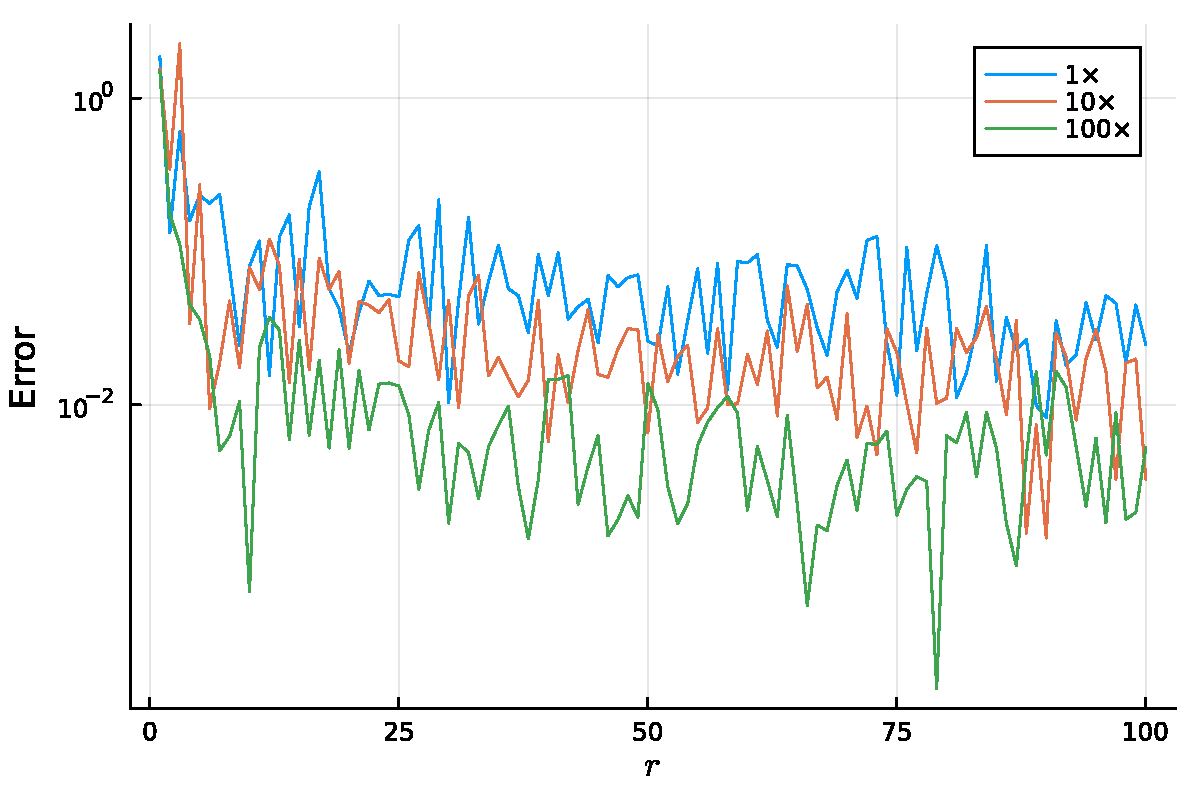
\includegraphics[width=0.6\linewidth,height=0.45\linewidth]{figures/IV.RandomisedLinearAlgebra_4_1.pdf}

That is to say, we can achieve accuracy to within about $1\%$ by solving 100 least squares problems involving $10 \ensuremath{\times} 2$ matrices.  I claim this is substantially faster, and so if $1\%$ accuracy suffices (which it does in \emph{many} applications) it is a big improvement.

\section{Poster projects}
We will leave further investigation of randomised linear algebra to posters:

\begin{itemize}
\item[1. ] How does the approximation property depend on the distribution of the sketch matrix? Can we use different sketch matrices to get better accuracy?


\item[2. ] What other algorithms are amenable to randomisation (trace estimation, low rank approximation, norm estimation, multiplication)?


\item[3. ] What applications are there to randomised linear algebra such as higher order polynomial regression?

\end{itemize}

